\section{Lp Spaces}

  Suppose $E$ is measurable, and $f$ is measurable on $E$. Then, define 
  \begin{equation}
    \|f\|_p \coloneqq \bigg( \int_E |f|^p \bigg)^{1/p}, \qquad 1 \leq p < +\infty
  \end{equation} 
  This tells us more about the properties of the function, and how it may blow up or how its singularities might behave. 

  For $p = \infty$, we can define it as the maximum of the function (since by EVT). In general, we can define 
  \begin{equation}
    \|f\|_{\infty} \coloneqq \mathrm{esssup} |f(x)| \coloneqq \inf \{ M \mid |f(x)| \leq M \text{ a.e. } x\}
  \end{equation}

  The functions in $L^p$ don't really satisfy the norm property that $\|f\| = 0 \iff f =0$, so we can just consider equivalence classes of functions. For the subadditivity of the norm, checking for $p=1$ is the easiest, and also to some extend $p=\infty$. 

  \begin{definition}[Lp Space]
    Given $1 \leq p \leq +\infty$, define $L^p (E)$ to be the vector space of all $f$ measurable on $E$ s.t. $\int_E |f|^p < +\infty$. 
  \end{definition}
  \begin{proof}
    We first prove that it is a linear space. Since 
    \begin{equation}
      | f + g |^p \leq 2^p (|f|^p + |g|^p)
    \end{equation}
    so $f + g \in L^p$ if $f, g \in L^p$. 
  \end{proof}

  \begin{theorem}[Young's Inequality]
    Suppose $1 \leq p < +\infty$, with $q = \frac{p}{p-1}$, i.e. $\frac{1}{p} + \frac{1}{q} = 1$. Let $a, b \geq 0$. Then 
    \begin{equation}
      a b \leq \frac{a^p}{p} + \frac{b^q}{q} 
    \end{equation}
  \end{theorem}
  \begin{proof}
    Let the exponential function be $y = x^{p-1}$. Then, we get $x = y^{\frac{1}{p-1}}$. The proof is similar to if the function intersects the upper side of the rectangle. 

    \begin{figure}[H]
      \centering
      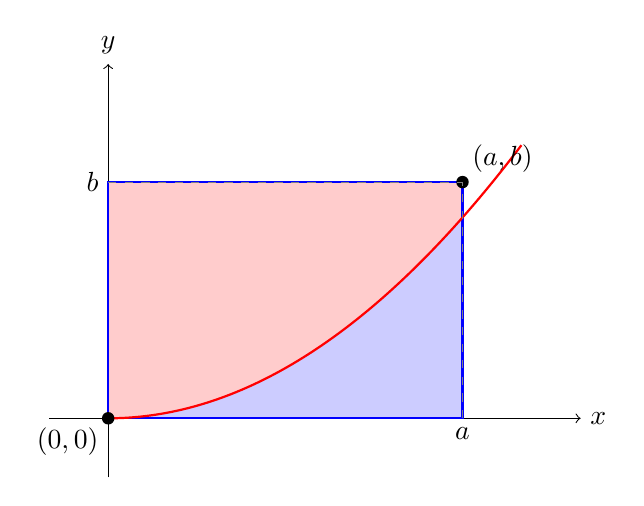
\begin{tikzpicture}[scale=1.5]
        % Draw axes
        \draw[->] (-0.5,0) -- (4,0) node[right] {$x$};
        \draw[->] (0,-0.5) -- (0,3) node[above] {$y$};
        
        % Define a and b
        \def\a{3}
        \def\b{2}
        
        % Shade area below the curve
        \fill[blue!20] (0,0) -- plot[domain=0:\a, samples=100] (\x, {1.7*(\x/\a)^2}) -- (\a,0) -- cycle;
        
        % Shade area above the curve
        \fill[red!20] plot[domain=0:\a, samples=100] (\x, {1.7*(\x/\a)^2}) -- (\a,\b) -- (0,\b) -- (0,0);
        
        % Draw rectangle
        \draw[blue, thick] (0,0) rectangle (\a,\b);
        
        % Draw exponential function extended beyond (a,b)
        \draw[red, thick, domain=0:3.5, samples=100] plot (\x, {1.7*(\x/\a)^2});
        
        % Label vertices
        \node[below left] at (0,0) {$(0,0)$};
        \node[above right] at (\a,\b) {$(a,b)$};
        
        % Mark points
        \fill (0,0) circle (1.5pt);
        \fill (\a,\b) circle (1.5pt);
        
        % Draw dashed lines to axes
        \draw[dashed, gray] (\a,0) -- (\a,\b);
        \draw[dashed, gray] (0,\b) -- (\a,\b);
        
        % Label axes values
        \node[below] at (\a,0) {$a$};
        \node[left] at (0,\b) {$b$};
      \end{tikzpicture}
      \caption{Rectangle with exponentially increasing curve and shaded regions}
      \label{fig:rectangle}
    \end{figure}

    We can see that the blue region has area 
    \begin{equation}
      \int_0^a x^{p-1} \,dx = \frac{a^p}{p} 
    \end{equation}
    We see that the red region has area $A$, 
    \begin{equation}
      A \leq \int_0^b y^{\frac{1}{p-1}} \,dy = \frac{y^{\frac{1}{p-1} + 1}}{\frac{1}{p-1} + 1} \bigg|_0^b = \frac{b^q}{q} 
    \end{equation}
  \end{proof}

  \begin{theorem}[Holder]
    Let $E$ be measurable, $1 \leq p \leq \infty$, $q = \frac{p}{p-1}$. Suppose $f \in L^p, g \in L^q$. Then, $f, g \in L^1 (E)$, and 
    \begin{equation}
      \int_E |fg| \,dx \leq \|f\|_p \|g\|_q
    \end{equation}
    In fact, this is sharp. If $f \neq 0$, then (note that this is the dual vector of $f$)
    \begin{equation}
      f^\ast (x) \coloneqq \|f\|_p^{1 - p} \mathrm{sgn}(f(x)) |f(x)|^{p-1} \in L^q
    \end{equation}
    with 
    \begin{equation}
      \|f^\ast \|_q = 1, \quad \int f f^\ast \,dx = \|f\|_p
    \end{equation}
  \end{theorem}
  \begin{proof}
    If $p =1$ ,or $p = \infty$, then this can be proven by monotonicity. If $1 < p < \infty$, then assume that $\|f\|_p = \|g\|_q = 1$, since by linearity, we can just normalize them by multiplying them by a constant. Not it suffices to prove that the integral $\leq 1$. Then, by Young's inequality,
    \begin{equation}
      |f(x) g(x)| \leq \frac{|f(x)|^p}{p} + \frac{|g(x)|^q}{q}
    \end{equation}
    and by integrating over $E$, since the RHS is integrable (it is also bounded?), we get 
    \begin{equation}
      \int_E |f(x) g(x)| \,dx \leq \frac{1}{p} + \frac{1}{q} = 1
    \end{equation}

    Finally, 
    \begin{equation}
      \|f^\ast\|_q^q = \|f\|_p^{(1-p) q} \int |f(x)|^{(p-1)q} \,dx = \|f\|_p^{-p} \int |f(x)|^p \,dx = 1
    \end{equation}
  \end{proof}

  \begin{corollary}[Cauchy-Schwartz]
    If $p = q = 2$, then we get Cauchy Schwartz. 
  \end{corollary}

  \begin{theorem}[Minkowski]
    If $f, g \in L^p$, then $f + g \in L^p$, and we get 
    \begin{equation}
      \| f + g \|_p \leq \|f\|_p + \|g\|_q
    \end{equation}
    This is the third condition for a norm. For $p = 1, +\infty$, this is immediate. Given $h \in L^p$, define 
    \begin{equation}
      h^\ast \coloneqq \|f\|_p^{1-p} \mathrm{sgn}(h) \, |h|^{p-1} 
    \end{equation}
    Then, from the previous theorem, 
    \begin{align}
      \| f + g \|_p & = \int_E (f + g)(f + g)^\ast \,dx  \\ 
                    & = \int_E f (f + g)^\ast \,dx + \int_E g (f + g)^\ast \,dx  \\ 
                    & \leq \|f\|_p \underbrace{\|(f + g)^\ast\|_q}_{1} + \|g\|_p \underbrace{\|(f + g)^\ast\|_q}_{1} 
    \end{align}
  \end{theorem}

  The following is an easy way to check that $\mathscr{F}$ is equi-integrable. 

  \begin{corollary}
    let $\mathscr{F}$ be a family of functions s.t. 
    \begin{equation}
      \int |f|^p \,dx < +\infty \forall f \in \mathscr{F}
    \end{equation}
    Then $\mathscr{F}$ is equi-integrable. 
  \end{corollary}
  \begin{proof}
    Let $A$ be ameasurable, $m(A) \leq \delta$. Then 
    \begin{equation}
      \int_A |f| \,dx \leq \bigg( \int_A |f|^p \bigg)^{1/p} \bigg( \int_A 1^q \bigg)^{1/q} \leq M^{1/p} m(A) \leq m^{1/p} \delta^{1/q} 
    \end{equation}
    Given any $\epsilon > 0$, we can choose $\delta > 0$ s.t. $\int |f| \,dx \leq \epsilon$ if $m(A) < \delta$. 
  \end{proof}

  \begin{corollary}
    Assume $E$ has finite measure. Then, $L^{p_1} \subset L^{p_2}$ for any $1 \leq p_1 \leq p_2 \leq +\infty$. So a higher exponent is more restrictive in a finite measure set. 
  \end{corollary}
  \begin{proof}
    A simple application of Holder's inequality. 
    \begin{equation}
      \int_E |f|^{p_1} \leq \bigg( \int_E |f|^{p_2} \,dx \bigg)^{p_1/p_2} x 
    \end{equation}
  \end{proof}

  In infinite measures, there are two ways that this can fail: singularities or tails. Either because it blows up, or it doesn't decay fast enough to be in $L^p$. $x^{-\alpha}$. 

\subsection{Nov 3} 

  \begin{example}
    Consider $f_m (x)$ in $L^p [0, 1]$, with 
    \begin{equation}
      f_m (x) =  \chi_{I_k^{(n)}} (x) \cdot 2^{n/p}, \quad I_k^{(n)} = [ (k-1) 2^{-n}, k 2^{-n}] 
    \end{equation}
    Note that $\|f_m\|_{L^p} = 1$, but $\|f_{m_1} - f_{m_2}\|_{L^p} \geq \frac{1}{2}$. So there are no limit points in $f_m$. 
  \end{example}

  \begin{definition}[Dual Vector]
    Suppose $X$ is a Banach space. Then $\mathcal{L}: X \to \mathbb{R}$ is called a \textbf{linear bounded functional} on $X$ if 
    \begin{equation}
      \mathcal{L}(\alpha f + \beta g)  = \alpha \mathcal{L} f + \beta \mathcal{L} g, \quad \forall f, g \in X
    \end{equation}
    and  
    \begin{equation}
      | \mathcal{L} (f)| \leq \|\mathcal{L}\|_\ast \|f\|, \quad \forall f \in X
    \end{equation}
  \end{definition}

  Whenever you want to prove that an integral is bounded, then you use Holder. 

  \begin{example}
    Let $X = L^p (E)$. Then 
    \begin{equation}
      \mathcal{L} f \coloneqq \int f g \,dx, \quad g \in L^q, q = \frac{p}{p - 1}
    \end{equation}
    is a linear bounded functional (by Holder). 
  \end{example}

  $L^\infty$ is not separable (as in there is no dense countable subset). 

  \begin{theorem}
    Given a Banach space $X$, the space of all linear bounded functionals on $X$ is a linear space with norm 
    \begin{equation}
      \|\mathcal{L}\|_\ast = \sup_{f \in X, \|f\| \leq 1} | \mathcal{L} (f) |
    \end{equation}
    This space is called \textbf{dual} to $X$, denoted $X^\ast$. 
  \end{theorem}
  \begin{proof}
    Just check that the sum, scalar multiplication is still a linear functional. Then for norm, just use triangle inequality. 
  \end{proof}

  We would like to prove that $(L^p)^\ast = L^q$, which we will do later. Now we'll define a different form of convergence. The regular pointwise convergence is known as strong convergence. 

  \begin{definition}[Weak Convergence]
    We say $f_n \rightharpoonup f$, i.e. \textbf{converges weakly} on $X$ if 
    \begin{equation}
      \mathcal{L}(f_n) \to \mathcal{L}(f), \quad \forall \mathcal{L} \in X^\ast
    \end{equation}
  \end{definition}


  \begin{example}
    Let $f_m(x)$ as before, and fix $g \in L^q [0, 1]$. Then, by Holder, 
    \begin{equation}
      \bigg| \int_0^1 \chi_{I_k^{(n)}} (x) g(x)\,dx  \bigg| \leq \|f_m\|_{L^p} \cdot \| g \cdot \chi_{I_k^{(n)}}\|_{L^q} \to 0, \text{ as } m \to +\infty
    \end{equation}
    since 
    \begin{equation}
      \int_{I_k^{(n)}} |g|^p \,dx \to 0 \text{ as } n \to +\infty
    \end{equation}
    by DCT, since $I_k^{(n)} = [(k-1) 2^{-n}, k 2^{-n}]$. 
  \end{example}

  So if we know that $(L^p)^\ast = L^q$, we could conclude $f_m \rightharpoonup 0$. 

  \begin{lemma}
    Suppose $\mathcal{L}_1, \mathcal{L}_2 \in X^\ast$. Suppose $Y$ is a dense subset of $X$. If $\mathcal{L}_1 = \mathcal{L}_2$ on $Y$, then $\mathcal{L}_1 = \mathcal{L}_2$. 
  \end{lemma}
  \begin{proof}
    Take any $g \in X$. Find $f \in Y$ s.t. $\|f - g\|_X \leq \epsilon$. Then, 
    \begin{align}
      |\mathcal{L}_1 g - \mathcal{L}_2 g| 
        & \leq |\mathcal{L}_1 g - \mathcal{L}_1 f| + \underbrace{|\mathcal{L}_1 f - \mathcal{L}_2 f|}_{=0} + |\mathcal{L}_2 f - \mathcal{L}_2 g| \\ 
        & \leq (\|\mathcal{L}_1\|_\ast + \| \mathcal{L}_2\|_\ast) \epsilon
    \end{align}
  \end{proof}

  \begin{lemma} 
    Let $E \subset \mathbb{R}$ be measurable, $1 \leq p \leq +\infty$. Suppose $g \in L^1 (E)$ and 
    \begin{equation}
      \bigg| \int_E f g \,dx \bigg| \leq M \| f\|_p, \quad \forall f \in L^p \text{ simple}
    \end{equation}
    Then, $g \in L^q, \|g\|_q \leq M$. 
  \end{lemma}
  \begin{proof}
    Consider $+\infty > p > 1$. Consider a sequence of simple $\varphi_n$ s.t. $\varphi_n \to |g|$ a.e., with $0 \leq \varphi_n \leq |g|$. Then, it suffices to show that 
    \begin{equation}
      \int | \varphi_n|^q \,dx \leq M, \quad \forall n
    \end{equation}
    since we can just invoke Fatou's lemma. Define simple $f_n = \mathrm{sgn}(g) |\varphi_n|^{q-1}$. Note $f_n \in L^p$ (simple functions). Then 
    \begin{equation}
      \int_E |\varphi_n|^q\,dx \leq  \int_E g \cdot f_n \,dx \leq M \|f_n \|_p, 
    \end{equation}
    where 
    \begin{equation}
      \|f_n\|_p = \bigg( \int | \varphi_n|^{q-1)p} \,dx \bigg)^{1/p} = \| \varphi_n \|_q^{q/p} 
    \end{equation}
    So $\| \varphi_n \|_q^{q- \frac{q}{p}} = \|\varphi_n\|_q \leq M$. Since $q(1 - \frac{1}{p}) = q \frac{1}{q} = 1$. 
  \end{proof}

  \begin{theorem}
    Let $[a, b]$ be a finite interval, with $1 \leq p < +\infty$. Suppose $\mathcal{L}$ is a linear bounded functional on $L^p([a, b])$. Then $\exists g \in L^q ([a, b])$ s.t. $\mathcal{L}f = \int_a^b f g \,dx$. 
  \end{theorem}
  \begin{proof}
    Suppose $p > 1$. Define $\phi(x) = \mathcal{L}(\chi_{[0, x]})$. We claim that $\phi$ is AC. Take $[a_k, b_k]_{k=1}^n$ disjoint in $[a, b]$. We have 
    \begin{equation}
      \sum_{k=1}^n |\phi(b_k) - \phi(a_k)|
    \end{equation}
    Given $\epsilon > 0$, we want to show that $\exists \delta >0$ s.t. 
    \begin{equation}
      \sum_{k=1}^n |b_k - a_k| \leq \delta \implies \sum_{k=1}^n |\phi(b_k) - \phi(a_k)| < \epsilon 
    \end{equation}
    But 
    \begin{align}
      \sum_{k=1}^n |\phi(b_k) - \phi(a_k)| & = \mathcal{L} \underbrace{\bigg( \sum_{k=1}^n \mathrm{sgn} \big( \phi(b_k) - \phi(a_k) \big) \chi_{[a_k, b_k]} \bigg)}_{f} \\ 
      & \leq \|\mathcal{L}\|_\ast \|f\|_p \\ 
      & = \|\mathcal{L}\|_\ast \bigg( \sum_{k=1}^n (b_k - a_k) \bigg)^{1/p}
    \end{align}
    Take $\delta = \big( \frac{\epsilon}{\|\mathcal{L}\|_\ast} \big)^{p}$
  \end{proof}

  So now that we have proved that $\phi$ is AC, we are almost in a position to use the lemma we proved before. Then, $\exists g \in L^1$ s.t. $\phi(x) = \int_a^x g(t) \,dt$ by fundamental theorem of calculus. Given ay $\chi_{[c, d]}$, we have 
  \begin{equation}
    \mathcal{L}(\chi_{c, d}) = \phi(d) - \phi(c) = \int_c^d g(t) \,dtjjA
  \end{equation}
  So $\mathcal{L} f$ and $\int g f \,dx$ coincide on step functions, and step functions are a dense set in $L^p$. We have 
  \begin{equation}
    \bigg| \int g f \,dx \bigg| \leq \|\mathcal{L}\|_\ast \|f\|_p 
  \end{equation}
  By the lemma, $g \in L^q$, with $\|g\|_q \leq \|\mathcal{L}\|_\ast$. 

  Note that this is \textit{not true} on $L^\infty$. Indeed $(L^1)^\ast = L^\infty$ (this is easier to prove), but $(L^\infty)^\ast \neq L^1$. But it is hard to construct a counterexample, and people use the Banach extension theorem to define such counterexamples. 

  \begin{theorem}[Riesz Representation Theorem]
    Let $E \subset \mathbb{R}$ be measurable, $1 \leq p < +\infty$. Suppose $\mathcal{L}$ is a bounded linear functional on $L^p$. Then $\exists g \in L^q$ s.t. 
    \begin{equation}
      \mathcal{L}(f) = \int_E g f \,dx, \quad \|g\|_q = \|\mathcal{L}\|_\ast
    \end{equation}
  \end{theorem}

  The dual of continuous functions is Steljes measures. 

  Now let's talk about weak convergence. This gives you some sort of compactness of a unit ball in $X^\ast$ with respect to the norm, which is basically sort of like weak convergence. 

  \begin{theorem}[Helley]
    Lt $X$ be a Banach space, separable. Suppose $\mathcal{L}_n \in X^\ast$ satisfy $\|L_n\|_\ast \leq M$ for all $n$. Then, $\exists n_k$ s.t. 
    \begin{equation}
      L_{n_k} (f) \to L (f), \quad \forall f \in X
    \end{equation}
  \end{theorem}
  \begin{proof}
    Let $(f_n)_{n=1}^\infty$ be a countable dense subset in $X$. Then, $\{\mathcal{L}_n f_1\}_{n=1}^\infty$ is ? $\implies \exists$ subsequence $s_{1, m}$ s.t. $\mathcal{L}_{s_{1, m}} f_1 \to a_1$. Also, we can choose a $s_{2, m}$ subsequence of $s_{1, m}$ s.t. $\mathcal{L}_{s_2, m} f_2 \to a_2$, and so in $s_{l, m}$ s.t. 
    \begin{equation}
      \mathcal{L}_{s_{l, m}} f_j \to a_j, \quad \forall 1 \leq j \leq l
    \end{equation}
    Select $n_k = S_{k, k}$. Then, $\mathcal{L}_{n_k} f_j \to a_j$ for all $j$. Given any $g \in X$, consider 
    \begin{equation}
      |\mathcal{L}_{n_{k_2}} g - \mathcal{L}_{n_{k_1}} g| \leq |\mathcal{L}_{n_{k_2}} g - \mathcal{L}_{n_{k_1}} f| + |\mathcal{L}_{n_{k_2}} f - \mathcal{L}_{n_{k_1}} f| + |\mathcal{L}_{n_{k_2}} f - \mathcal{L}_{n_{k_1}} g|
    \end{equation}
    Fix $\epsilon > 0$, choose $f$ s.t. 
    \begin{equation}
      \|f - g\| \leq \frac{\epsilon}{3 \max\{\|f\|, \|g\|\}}
    \end{equation}
    Then, $k_1, k_2$, large so middle term $\leq \frac{\epsilon}{3}$. 
  \end{proof}

  So this is what people mean by a unit ball in $L^p$ is weakly compact. 

\subsection{Exercises} 

  \begin{exercise}[Math 631 Fall 2025, Final Exam Exercise 6]
    Define $c_{0}$ to be a space of all sequences $x=x_{1},x_{2},...,x_{n},...$ that converge to zero, with the norm $\|x\|=\sup_{n}|x_{n}|$. Prove that $c_{0}$ is a Banach space and find its dual.
  \end{exercise}
  \begin{solution}
    Suppose that $x^{m}$ is a Cauchy sequence in $c_{0}$. Then each component $x_{n}^{m}$ is also a Cauchy sequence of real numbers, and converges to some $y_{n}$. It is not hard to see that $y_{n}$ is a bounded sequence: take $\epsilon=1$ and find $N$ such that $\|x^{m}-x^{N}\|_{\infty}\le1$ if $m\ge N$. Then also $\|y-x^{N}\|_{\infty}\le1$, and so $y\in l^{\infty}$. Let us now show that $y\in c_{0}$. Fix $\epsilon>0$. Find $N$ such that $\|y-x^{N}\|_{\infty}\le\epsilon/2$. Next, since $x^{N}\in c_{0}$, find $M$ such that $|x_{m}^{N}|\le\epsilon/2$ for all $m\ge M$. Then for every $m\ge M$,
    \begin{equation}
      |y_{m}|\le|y_{m}-x_{m}^{N}|+|x_{m}^{N}|\le\epsilon.
    \end{equation}
    Hence $y\in c_{0}$. This proves $c_{0}$ is a Banach space.

    Take any sequence $a_{n}$ in $l_{1}$, then it defines a bounded linear functional $A$ on $c_{0}$ defined by $A(x)=\sum_{n=1}^{\infty}a_{n}x_{n}$. Note that $\|A\|=\|a\|_{l^{1}}$: we can just take sequences $x_{n}^{m}$ that take value 1 if $a_{n}>0$ and -1 if $a_{n}<0$ for $n=1,...,m$. Then $\|x^{m}\|_{\infty}=1$, and
    \begin{equation}
      \sum_{n=1}^{\infty}a_{n}x_{n}^{m}\rightarrow\|a\|_{l^{1}}
    \end{equation}
    as $m\rightarrow\infty$ by Lebesgue dominated convergence theorem. On the other hand, let $A$ be any bounded linear functional on $c_{0}$. For every $n$, take $e^{n}\in c_{0}$ such that $e_{j}^{n}=\delta_{nj}$ (1 if $j=n$ and 0 if $j\ne n$). Set $a_{n}=A(e_{n})$. By taking $x^{m}$ before equal to $\pm1$ depending on the sign of $a_{n}$ for the first $m$ positions, we find that
    \begin{equation}
      A(x^{m})=\sum_{n=1}^{m}|a_{n}|\le\|A\|,
    \end{equation}
    for every $m$. Therefore, $a_{n}\in l^{1}$ and then it is not hard to see $\|A\|=\|a\|_{l^{1}}$. Hence the dual space of $c_{0}$ can be identified with $l^{1}$.
  \end{solution}

  \begin{exercise}[Math 631 Fall 2025, Final Exam Exercise 7]
    Let $h$ be continuous function periodic on $\mathbb{R}$ with period one, and assume $\int_{0}^{1}h(x)dx=0$. Define $f_{n}(x)=h(nx)$. Show that for any finite interval $[a, b]$, $f_{n}\rightarrow0$ in $L^{p}[a,b]$, $1\le p<\infty$.
  \end{exercise}
  \begin{solution}
    Since step functions are dense in $L^{p}[a,b]$, it suffices to prove that for any $a\le c < d\le b,$ $\int_{c}^{d}h(nx)dx\rightarrow0$ as $n\rightarrow\infty$. But
    \begin{equation}
      \int_{c}^{d}h(nx)dx=n^{-1}\int_{nc}^{nd}h(y)dy\le2\|h\|_{L^{\infty}}n^{-1}\rightarrow0
    \end{equation}
    as $n\rightarrow\infty$. Here we used that periodic continuous function must be bounded, and integrated over all full periods included into $[nc, nd]$ getting zero from these parts since $h$ is mean zero.
  \end{solution}

